\section{Materiais e métodos}
\subsection{Materiais}
\subsubsection{qPCR e High Resolution Melting Analysis}
     
\subsection{Métodos}
\subsubsection{qPCR e High Resolution Melting Analysis}

\begin{wrapfigure}{r}{.45\textwidth}
    \centering
    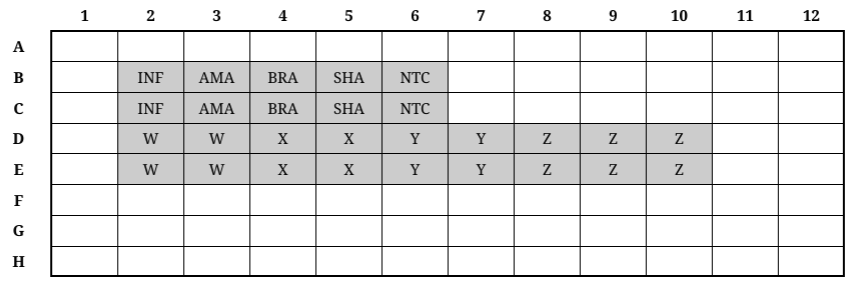
\includegraphics[width=.4\textwidth]{fig/placa_org.png}
    \caption{Disposição das soluções de reação na placa de 96 poços para qPCR. Os poços em branco estão vazios, os poços com solução estão nomeados de acordo com a amostra de DNA. INF - \textit{L. infantum}; AMA - \textit{L. amazonensis}; BRA \textit{L. braziliensis}; SHA - \textit{L. shawi}; NTC - controle negativo; W, X, Y e Z são amostras desconhecidas.}
    \label{wellorg}
\end{wrapfigure}

O protocolo foi adaptado de Zampieri et.al.\cite{HRMzampi2016}.
Foram preparados 28 soluções de \qty{20}{\micro\liter} com
\qty{10}{\micro\liter} de
MeltDoctorTM HRM Master Mix (Thermo fischer Scientific), \qty{0,6}{\micro\liter} de
Primer hsp70-F2, \qty{0,6}{\micro\liter} de Primer hsp70C-R,
\qty{6,3}{\micro\liter} de
água e \qty{2,5}{\micro\liter} de amostra de DNA genômico. Destas 28 soluções,
oito receberam como amostra controle positivo, sendo duas de \textit{L. (L.)
infantum}, duas de \textit{L. (L.) amazonensis}, duas de \textit{L. (V.)
braziliensis} e duas de \textit{L. (V.) shawi}. Duas das soluções receberam
controle negativo, sem DNA genômico. O restante das soluções receberam as
amostras desconhecidas denominadas amostras W, X, Y, Z, sendo quatro soluções de
cada amostra. As soluções foram distribuídas em uma placa de 96 poços conforme a
\cref{wellorg}. A reação de qPCR foi realizada no equipamento StepOne System
(Thermo Fischer Scientific). Primeiro foi feita incubação à \qty{94}{\celsius}
por 5 minutos.  Então, a reação foi submetida à 40 ciclos de desnaturação à
\qty{94}{\celsius} por 30 s, associação e extensão a \qty{60}{\celsius} por 30s. 

